\begin{multicols}{2}

\usetikzlibrary{shapes,positioning}

\newcommand{\foo}{\hspace{-2.3pt}$\bullet$ \hspace{5pt}}

\interesting{A timeline details design iteration throughout the season}{timeline:1}

\raggedleft

\newcounter{year}
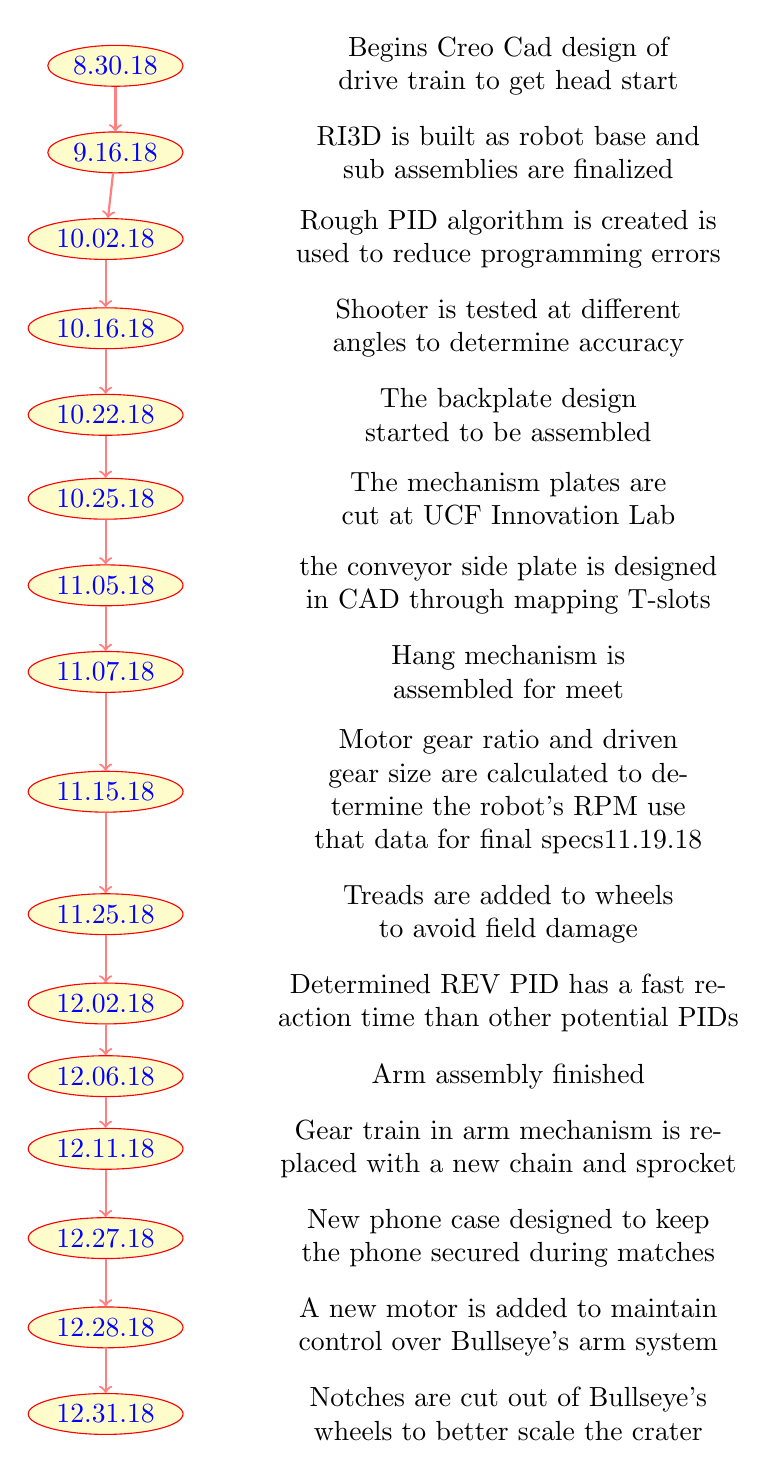
\begin{tikzpicture}[yscale=0.5,%
           year/.style={draw=red,text=blue,fill=yellow!20,shape=ellipse,inner sep=2pt},
           description/.style={rectangle,align=center,text width=60mm,anchor=west},
           timeline/.style={->,thick,red!50}]

    \foreach \year/\desc [count=\y] in {%
       8.30.18/Begins Creo Cad design of drive train to get  head start,
       9.16.18/RI3D is built as robot base and sub assemblies are finalized,%
       10.02.18/Rough PID algorithm is created is used to reduce programming errors,%
       10.16.18/Shooter is tested at different angles to determine accuracy,%
       10.22.18/The backplate design started to be assembled,%
       10.25.18/The mechanism plates are cut at UCF Innovation Lab,%
       11.05.18/the conveyor side plate is designed in CAD through mapping T-slots,%
       11.07.18/Hang mechanism is assembled for meet,%
       11.15.18/Motor gear ratio and driven gear size are calculated to determine the robot's RPM use that data for final specs%
       11.19.18/Big wheel drive train begans to go through design process,%
       11.25.18/Treads are added to wheels to avoid field damage,%
       12.02.18/Determined REV PID has a fast reaction time than other potential PIDs,%
       12.06.18/Arm assembly finished,%
       12.11.18/Gear train in arm mechanism is replaced with a new chain and sprocket,%
       12.27.18/New phone case designed to keep the phone secured during matches,%
       12.28.18/A new motor is added to maintain control over Bullseye’s arm system,%
       12.31.18/Notches are cut out of Bullseye’s wheels to better scale the crater%
       } { \ifnum\y=1 \node[description](\y){\desc};
           \else\node[description,below=1ex of \z](\y){\desc};
           \fi
           \node[year](y-\y) [left=of \y] {\year};
           \ifnum\y>1\draw[timeline] (y-\z)-- (y-\y);\fi
           \global\let\z=\y% for drawing from last node
       }




\end{tikzpicture}

\columnbreak

\raggedleft
\begin{center}
        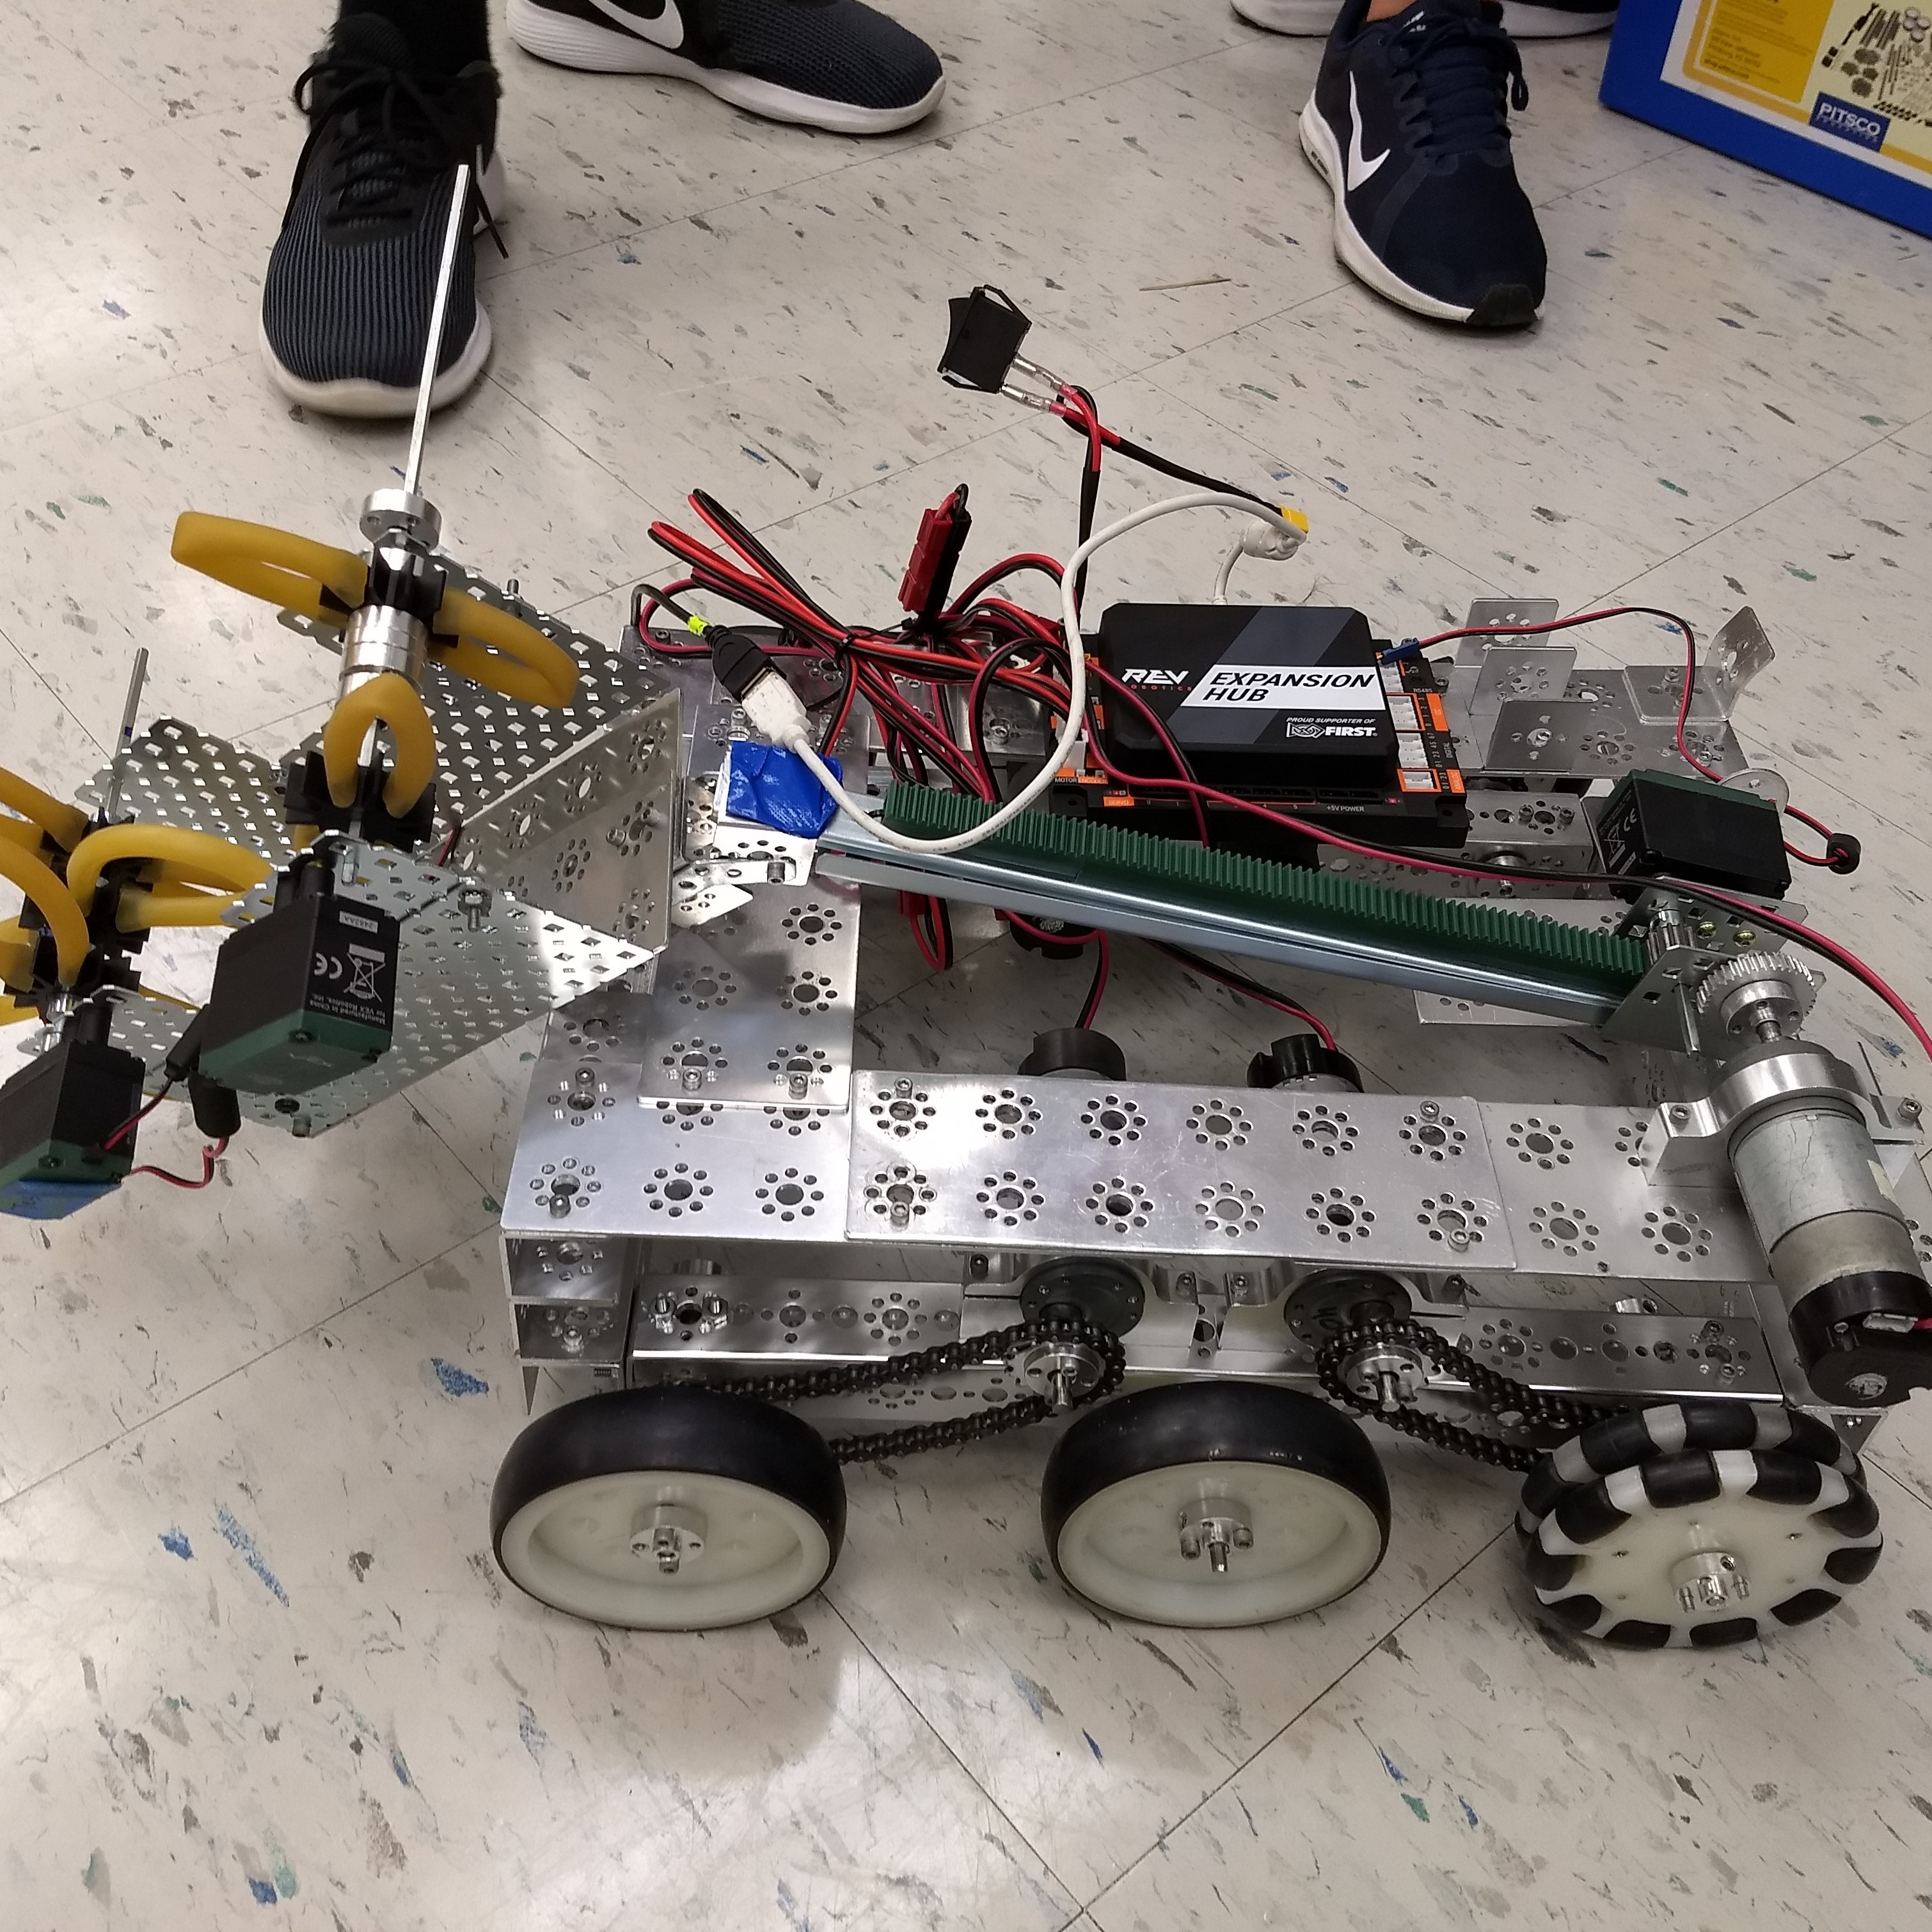
\includegraphics[width=.13\textwidth]{Design_Overview/timephoto1.jpg}
\end{center}
\begin{center}
        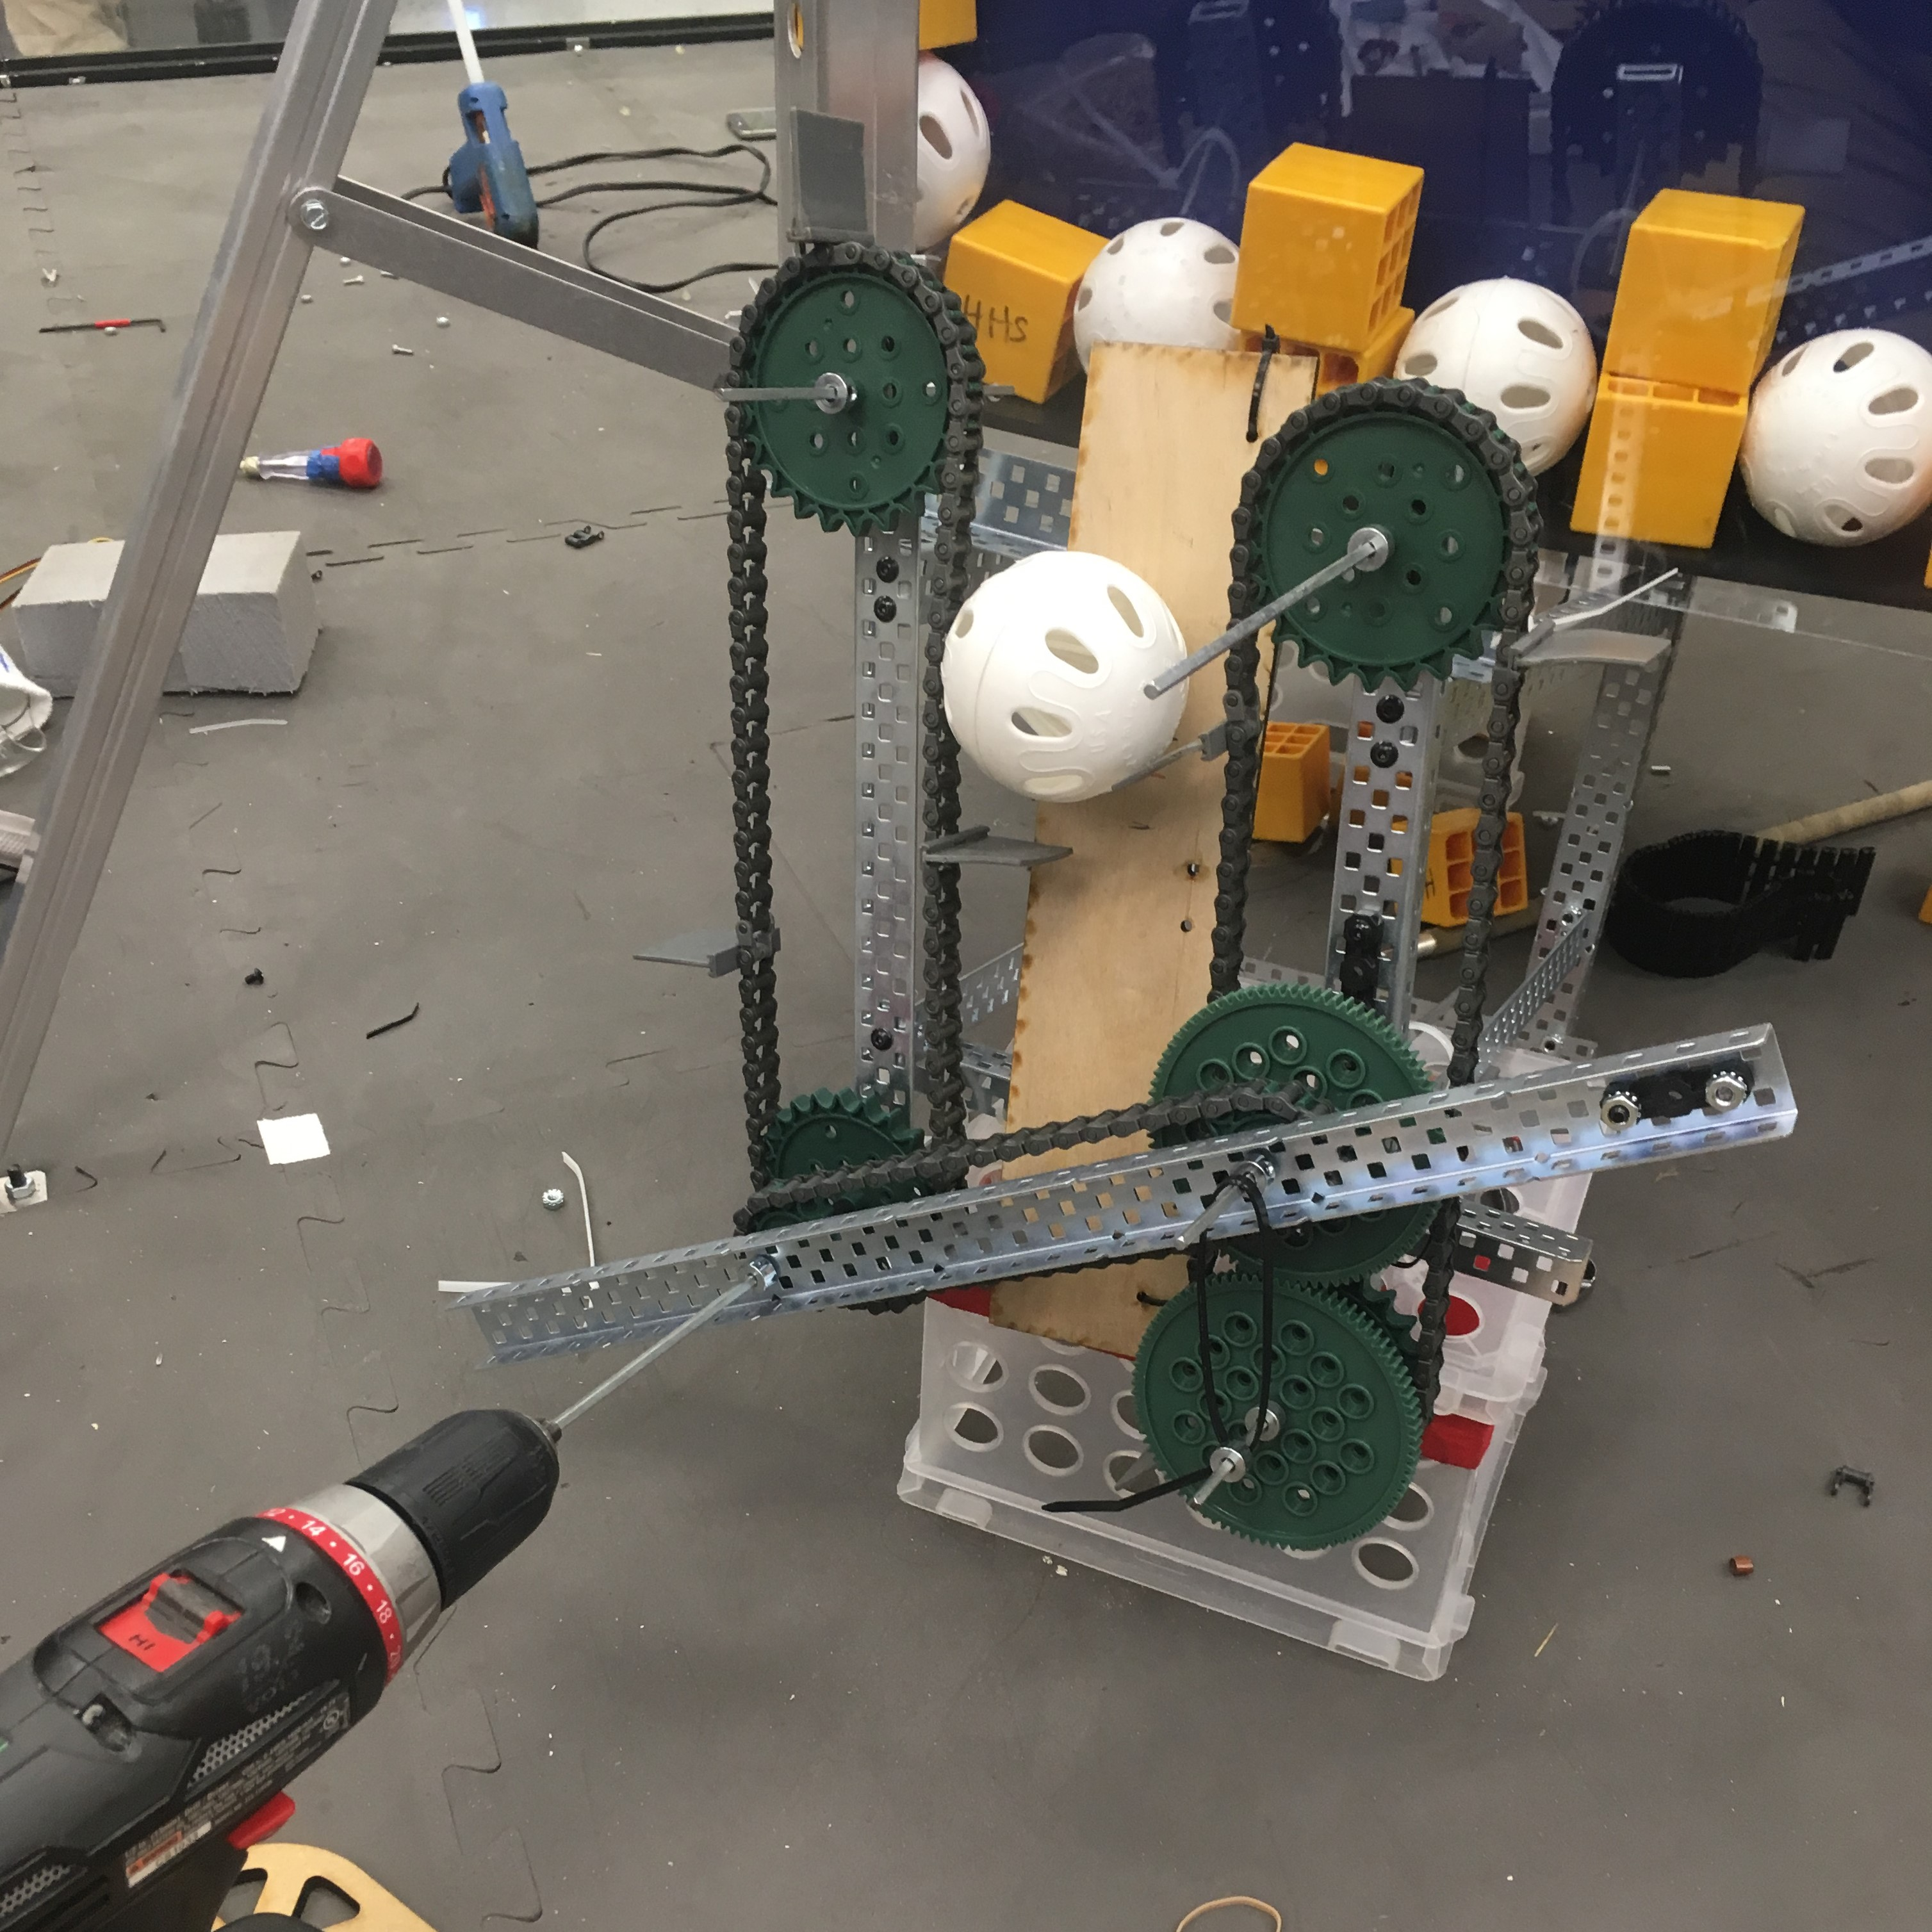
\includegraphics[width=.13\textwidth]{Design_Overview/timephoto2.JPG}
\end{center}
\begin{center}
        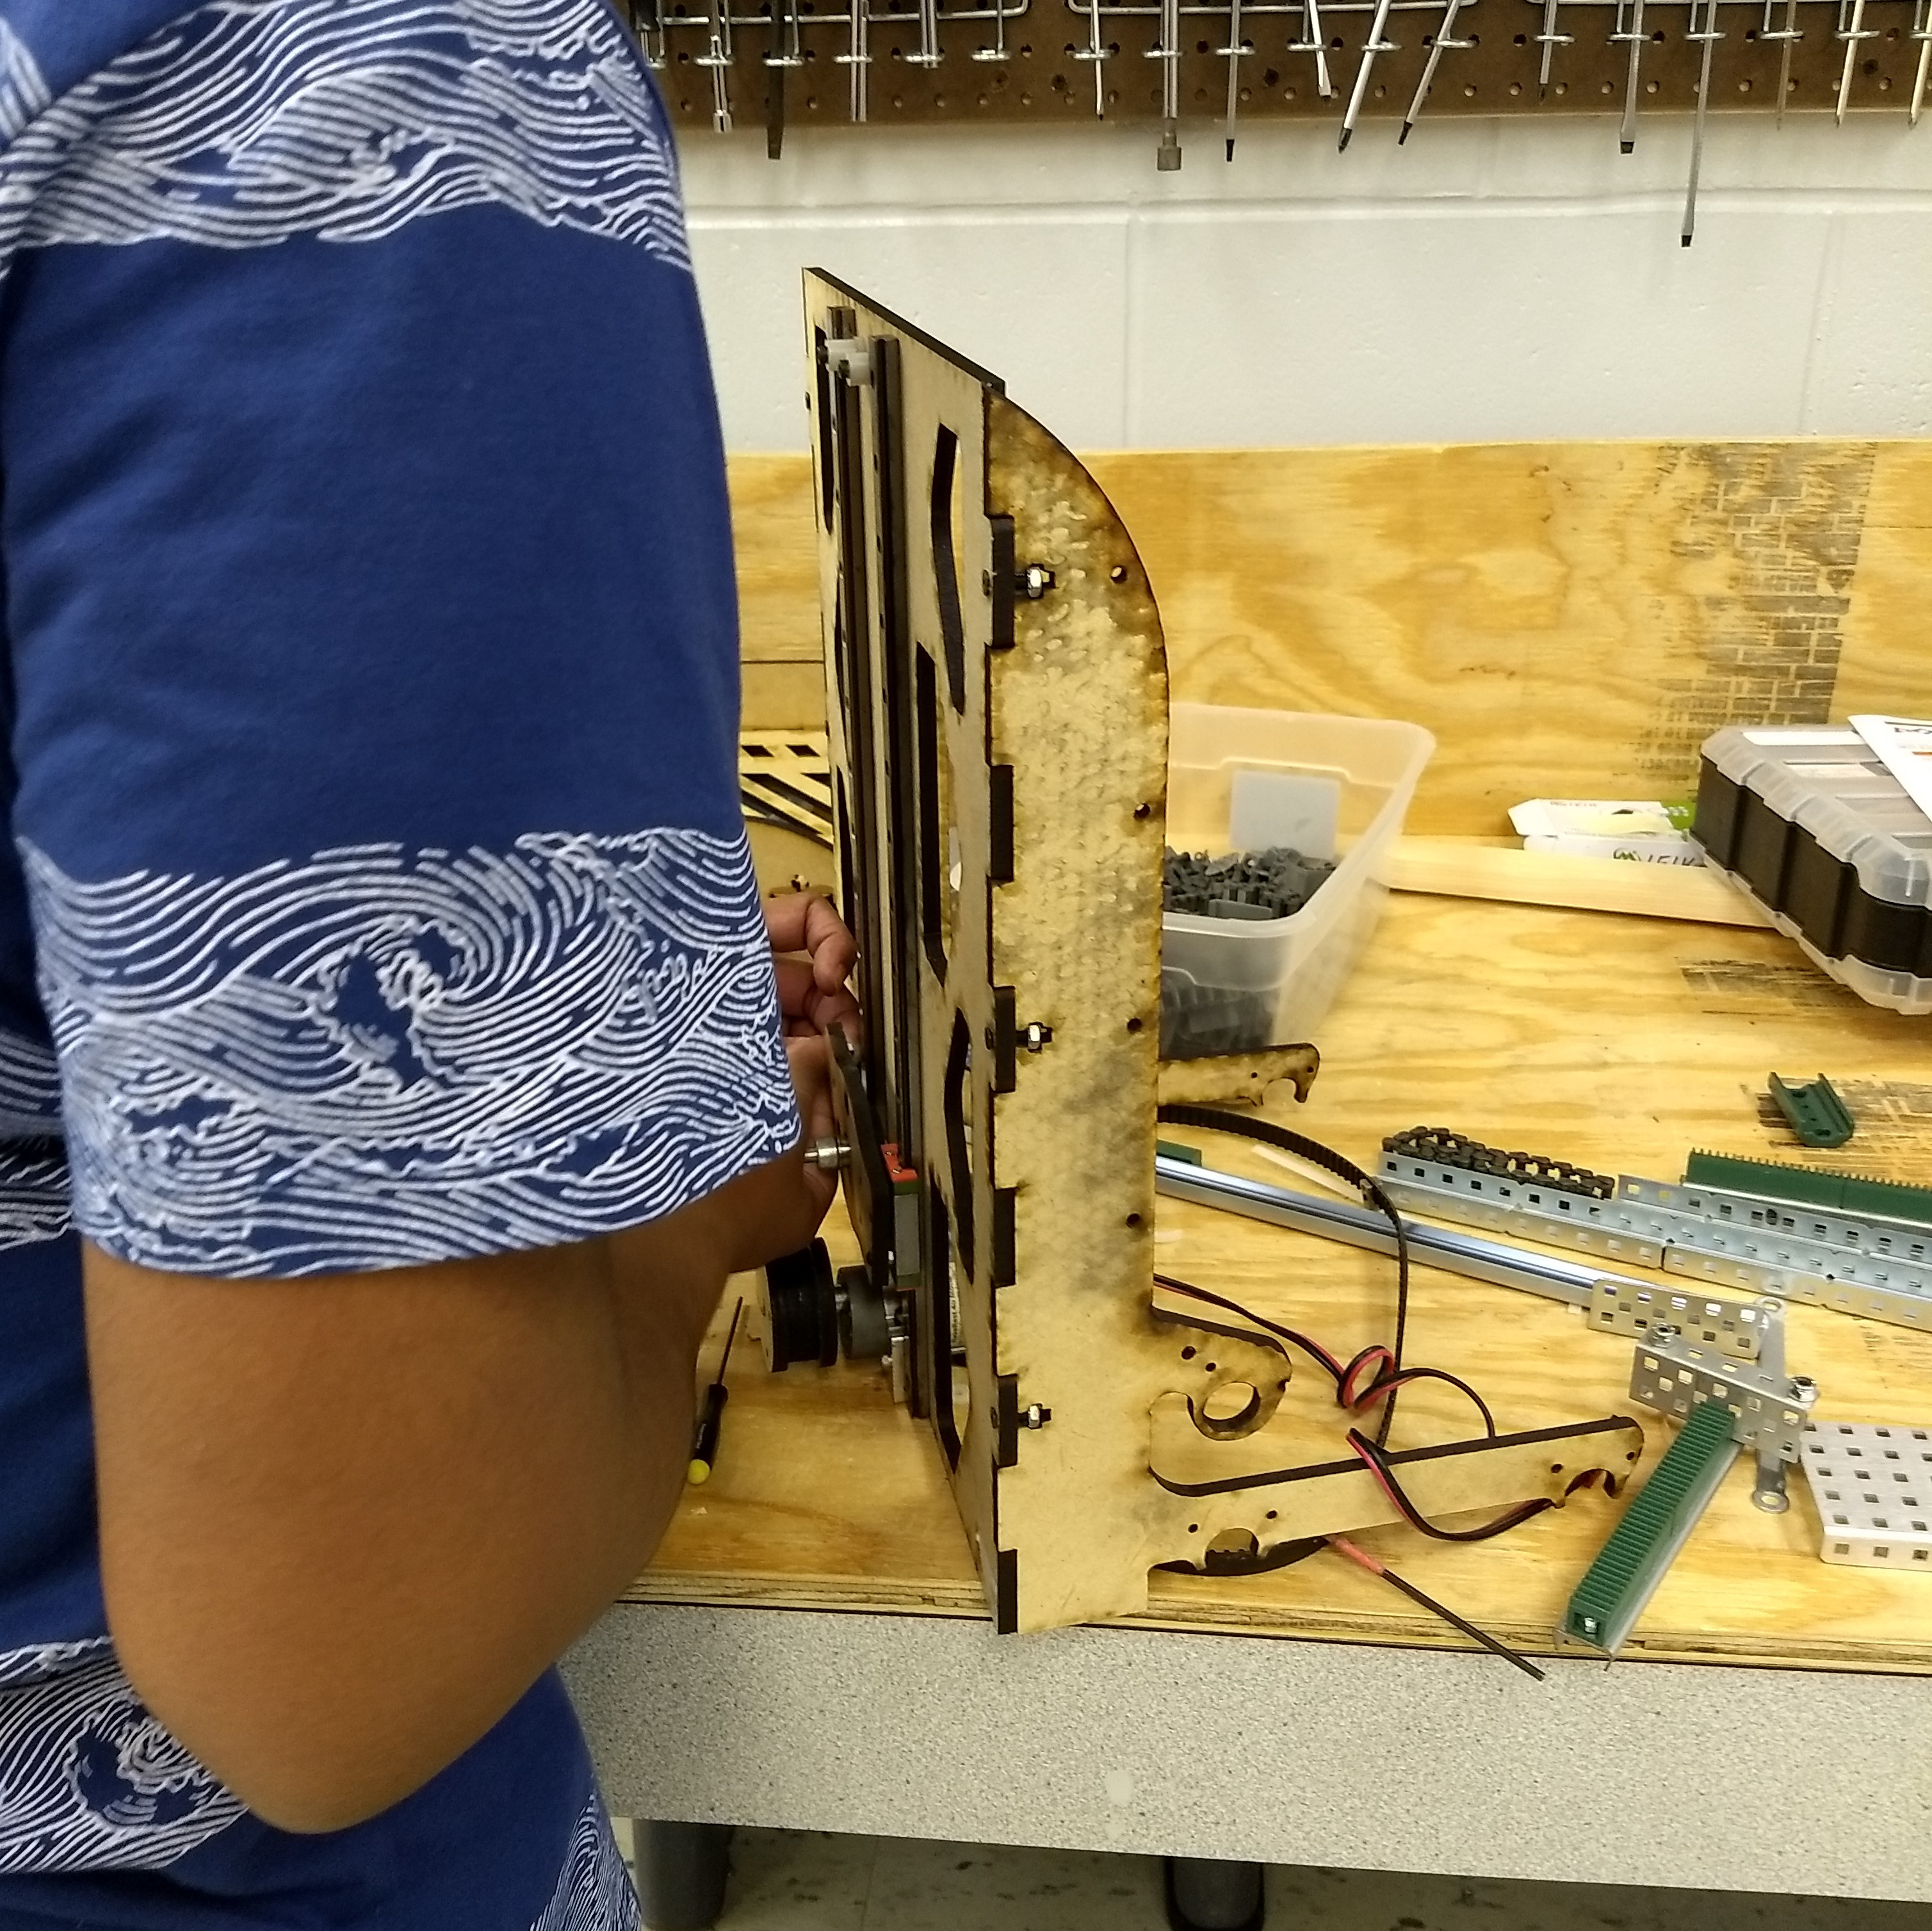
\includegraphics[width=.13\textwidth]{Design_Overview/timephoto3.jpg}
\end{center}
\begin{center}
        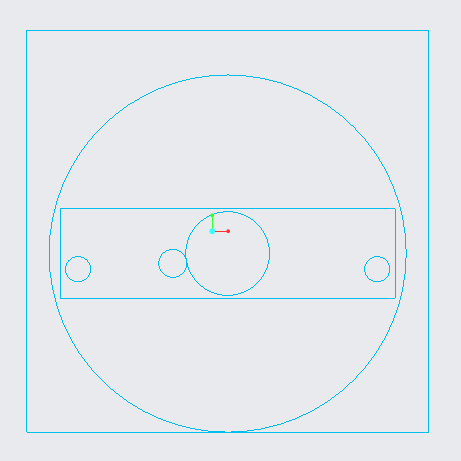
\includegraphics[width=.13\textwidth]{Design_Overview/timephoto5.PNG}
\end{center}
\begin{center}
        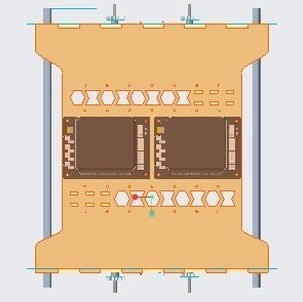
\includegraphics[width=.13\textwidth]{Design_Overview/timephoto7.JPG}
\end{center}
\begin{center}
        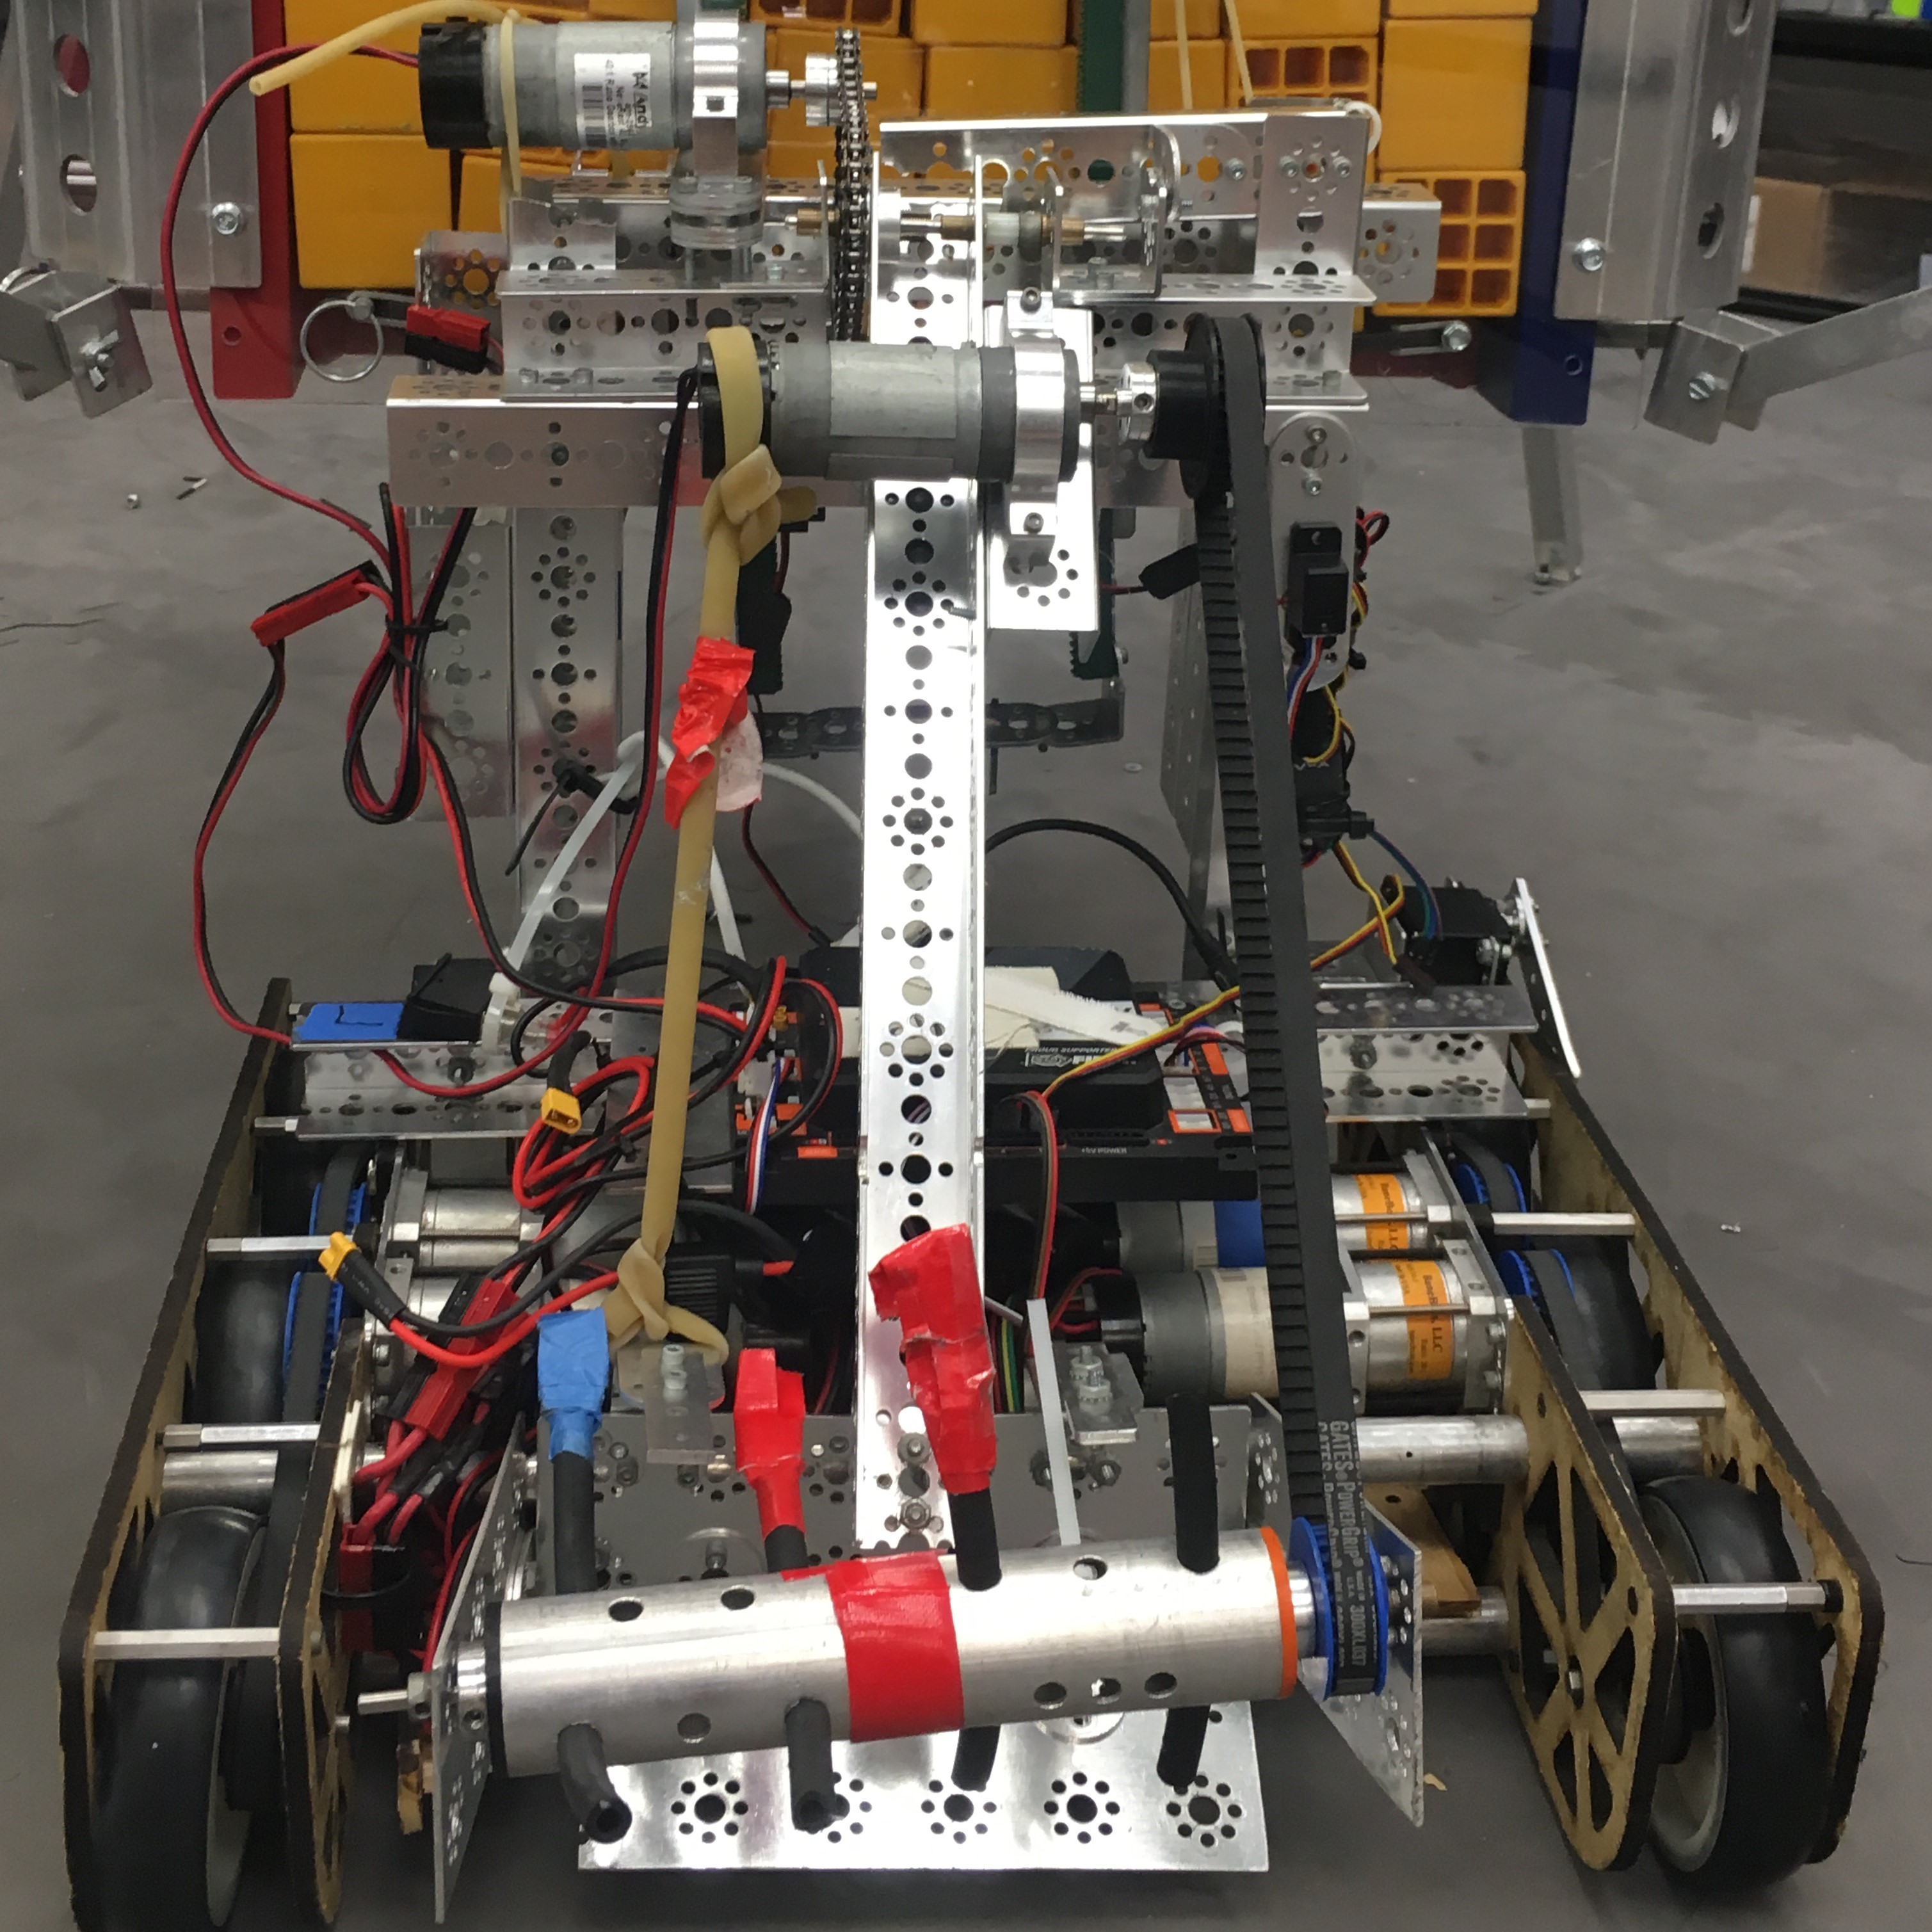
\includegraphics[width=.13\textwidth]{Design_Overview/timephoto8.JPG}
\end{center}
\begin{center}
        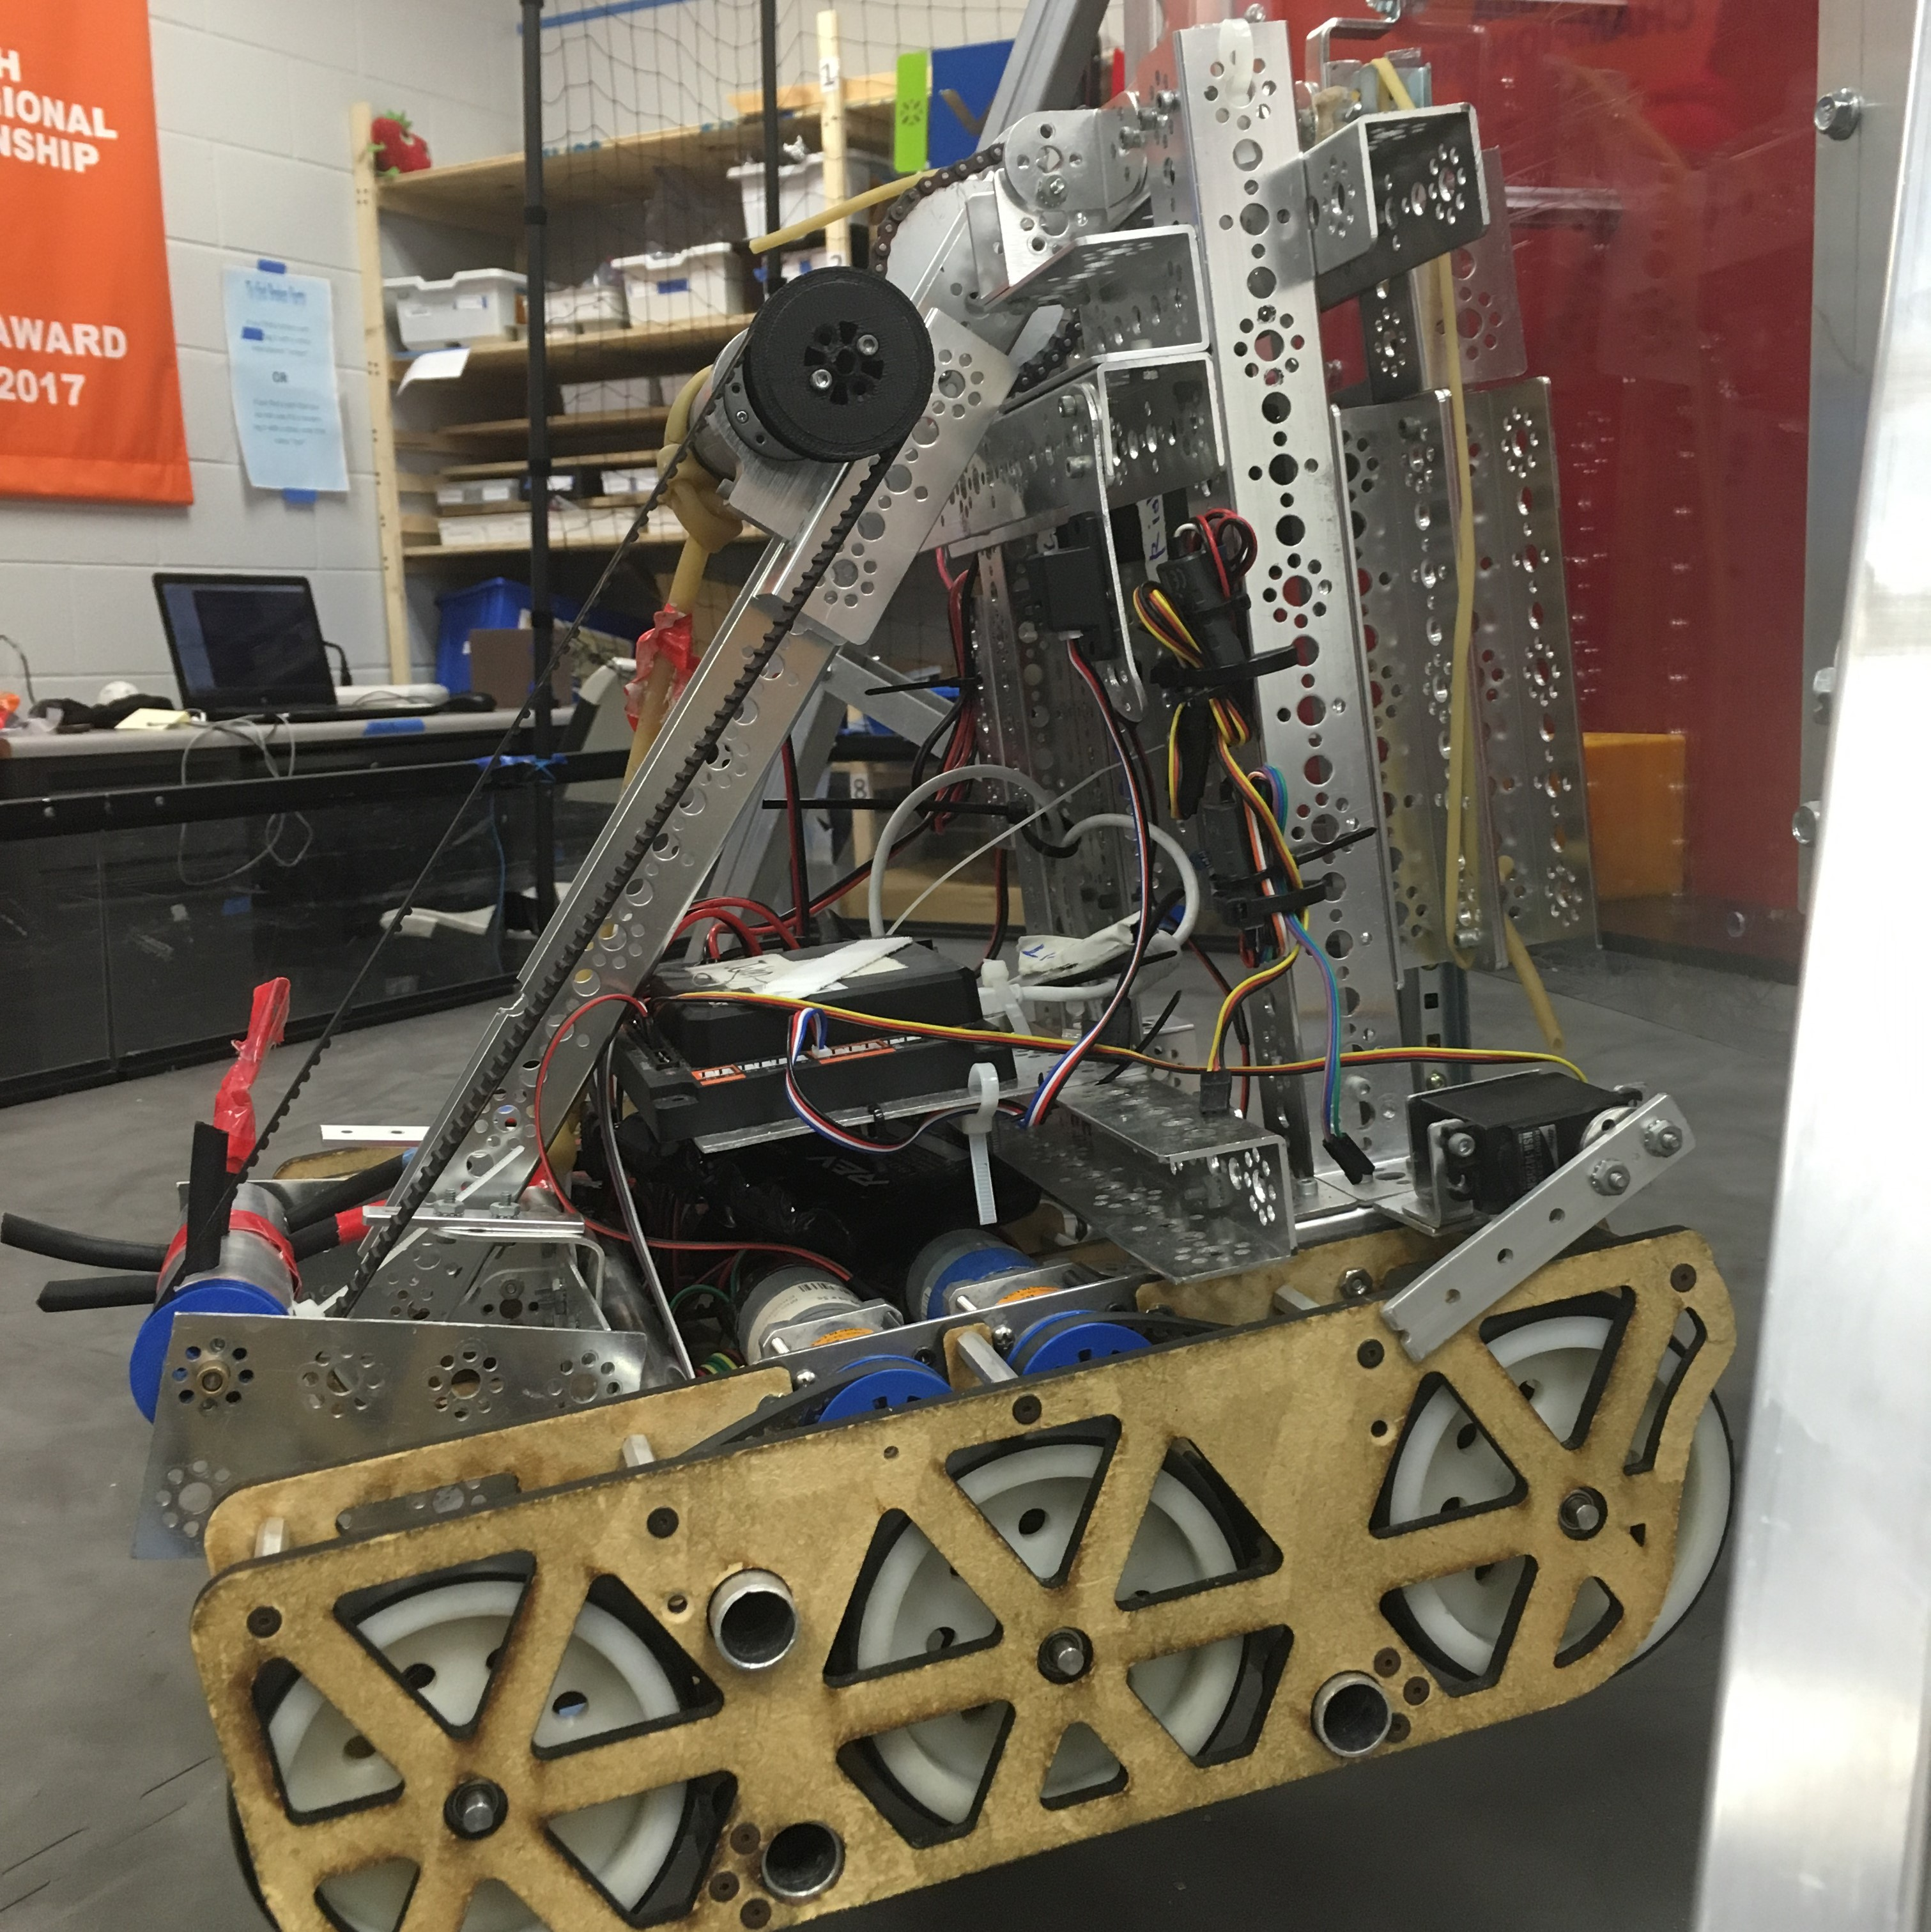
\includegraphics[width=.13\textwidth]{Design_Overview/timephoto9.png}
\end{center}
\begin{center}
        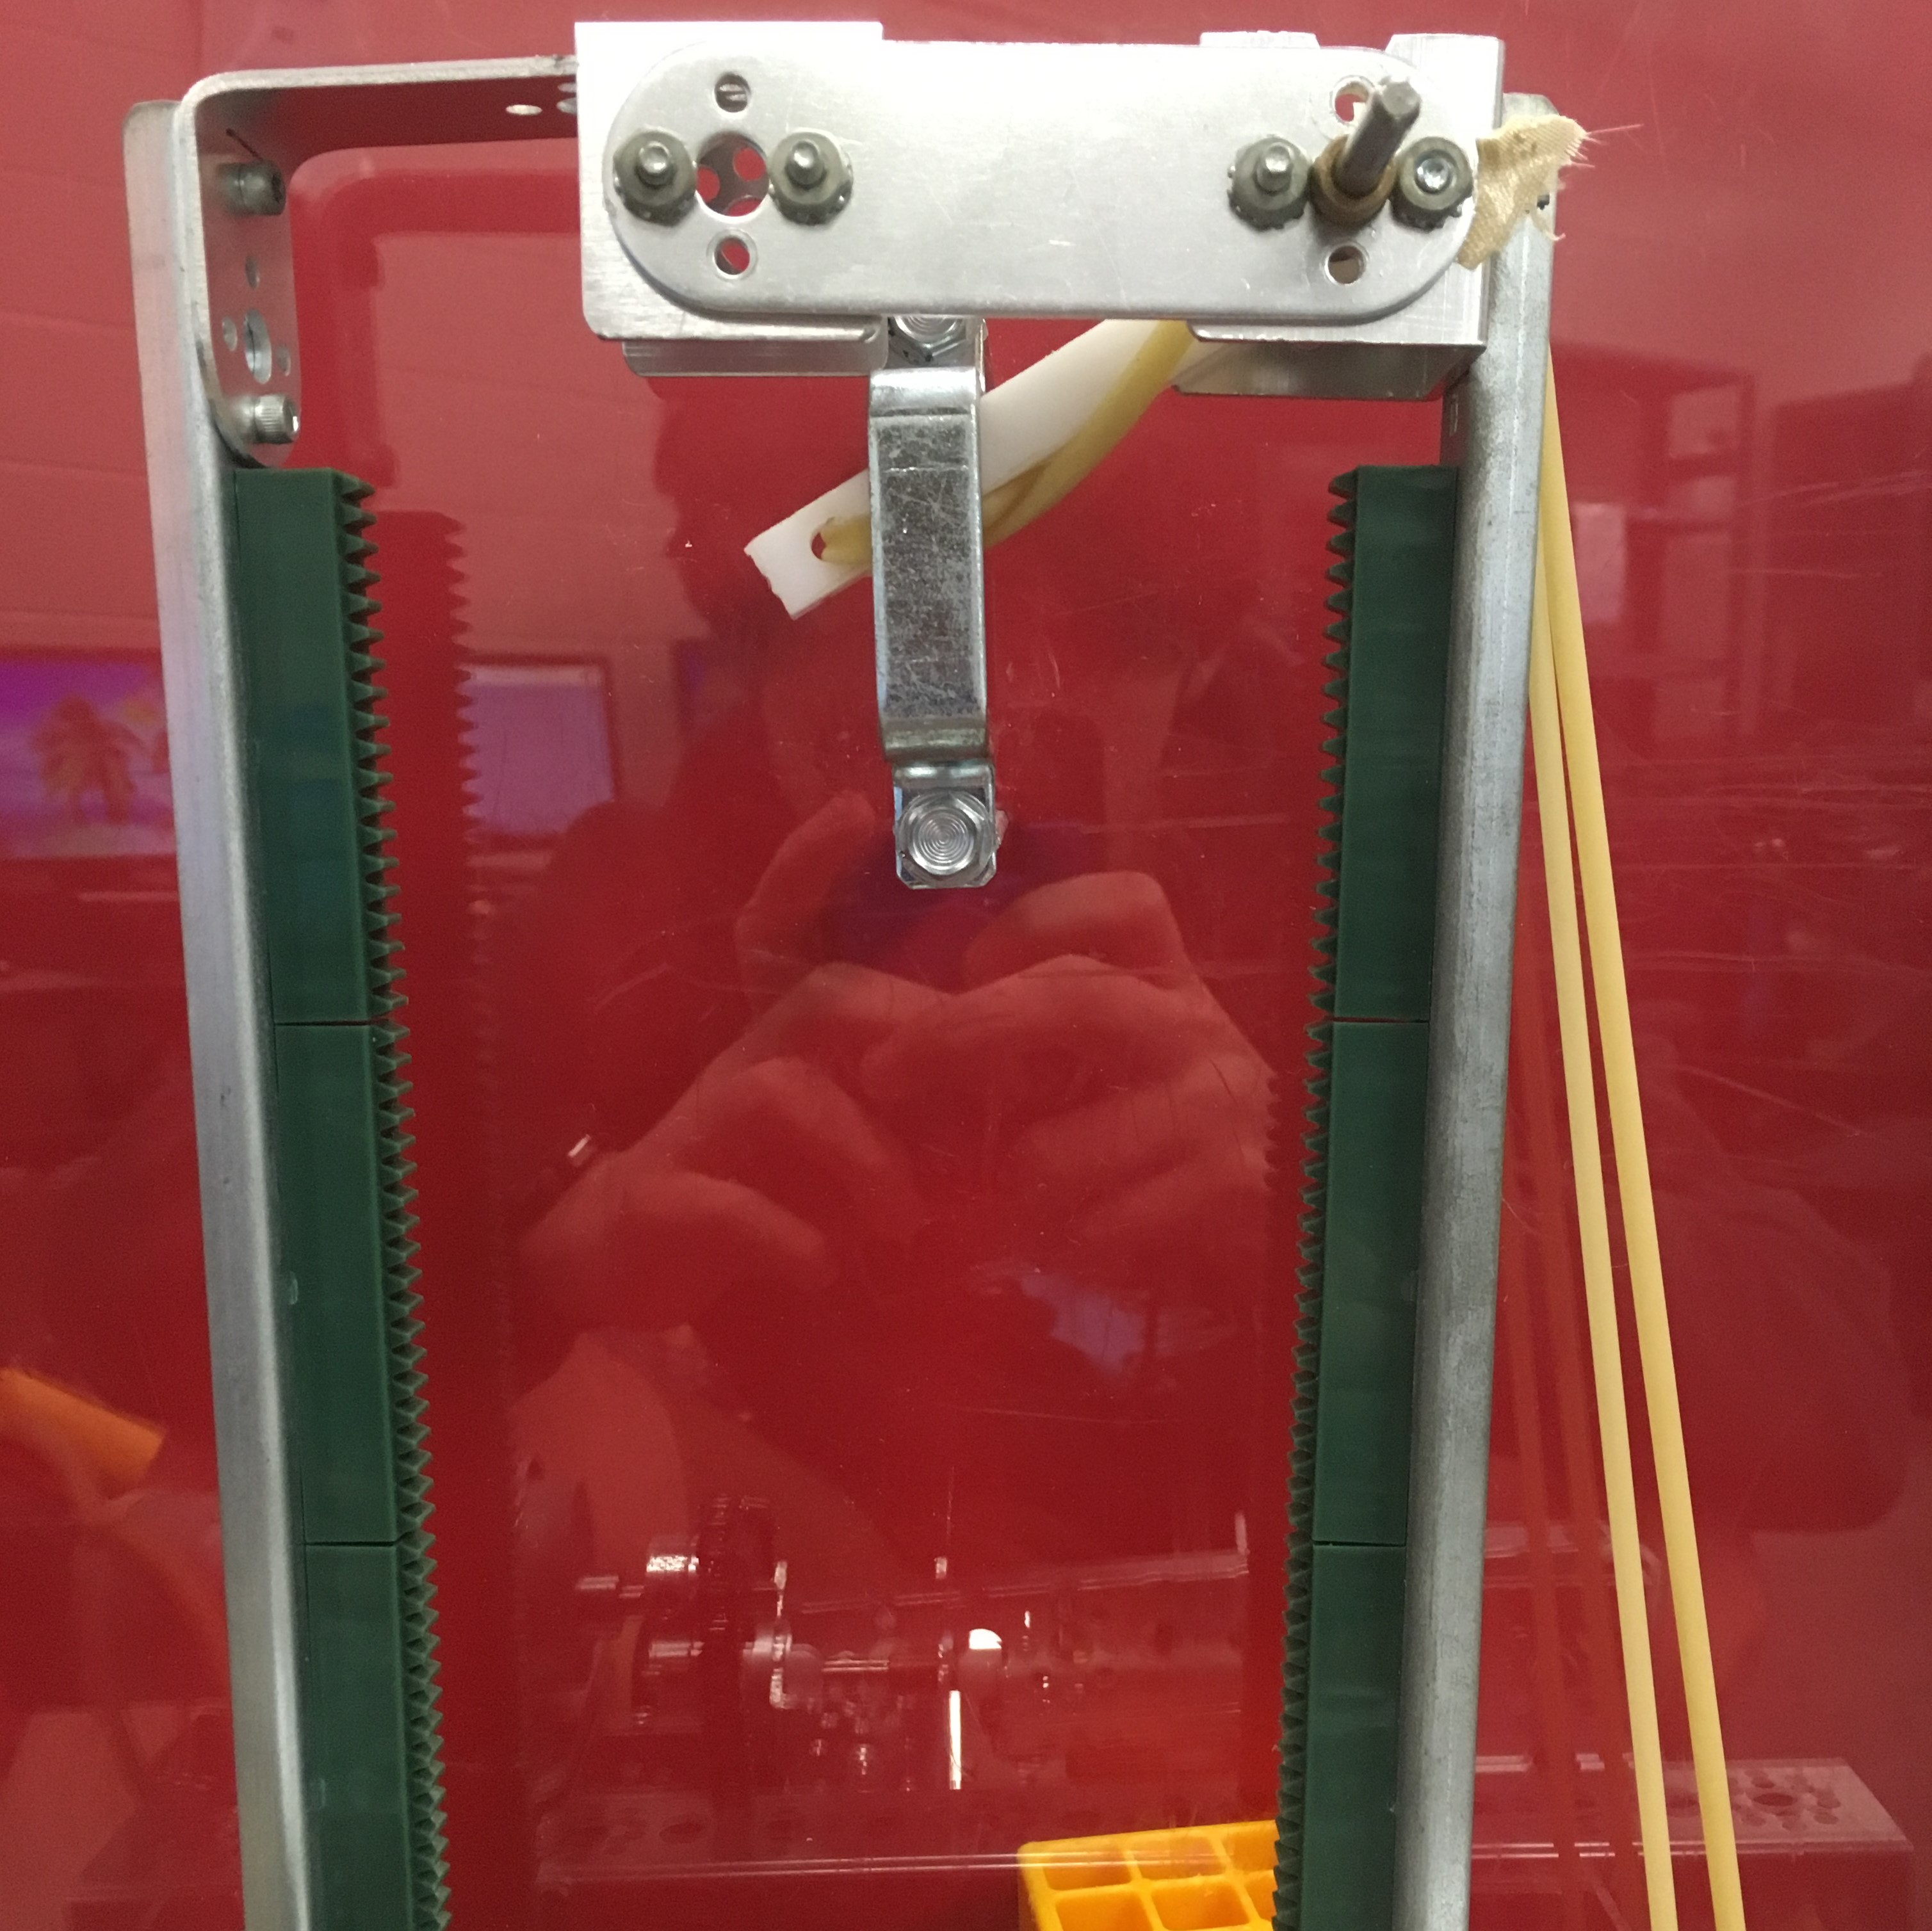
\includegraphics[width=.13\textwidth]{Design_Overview/timephoto9-5.png}
\end{center}
\begin{center}
        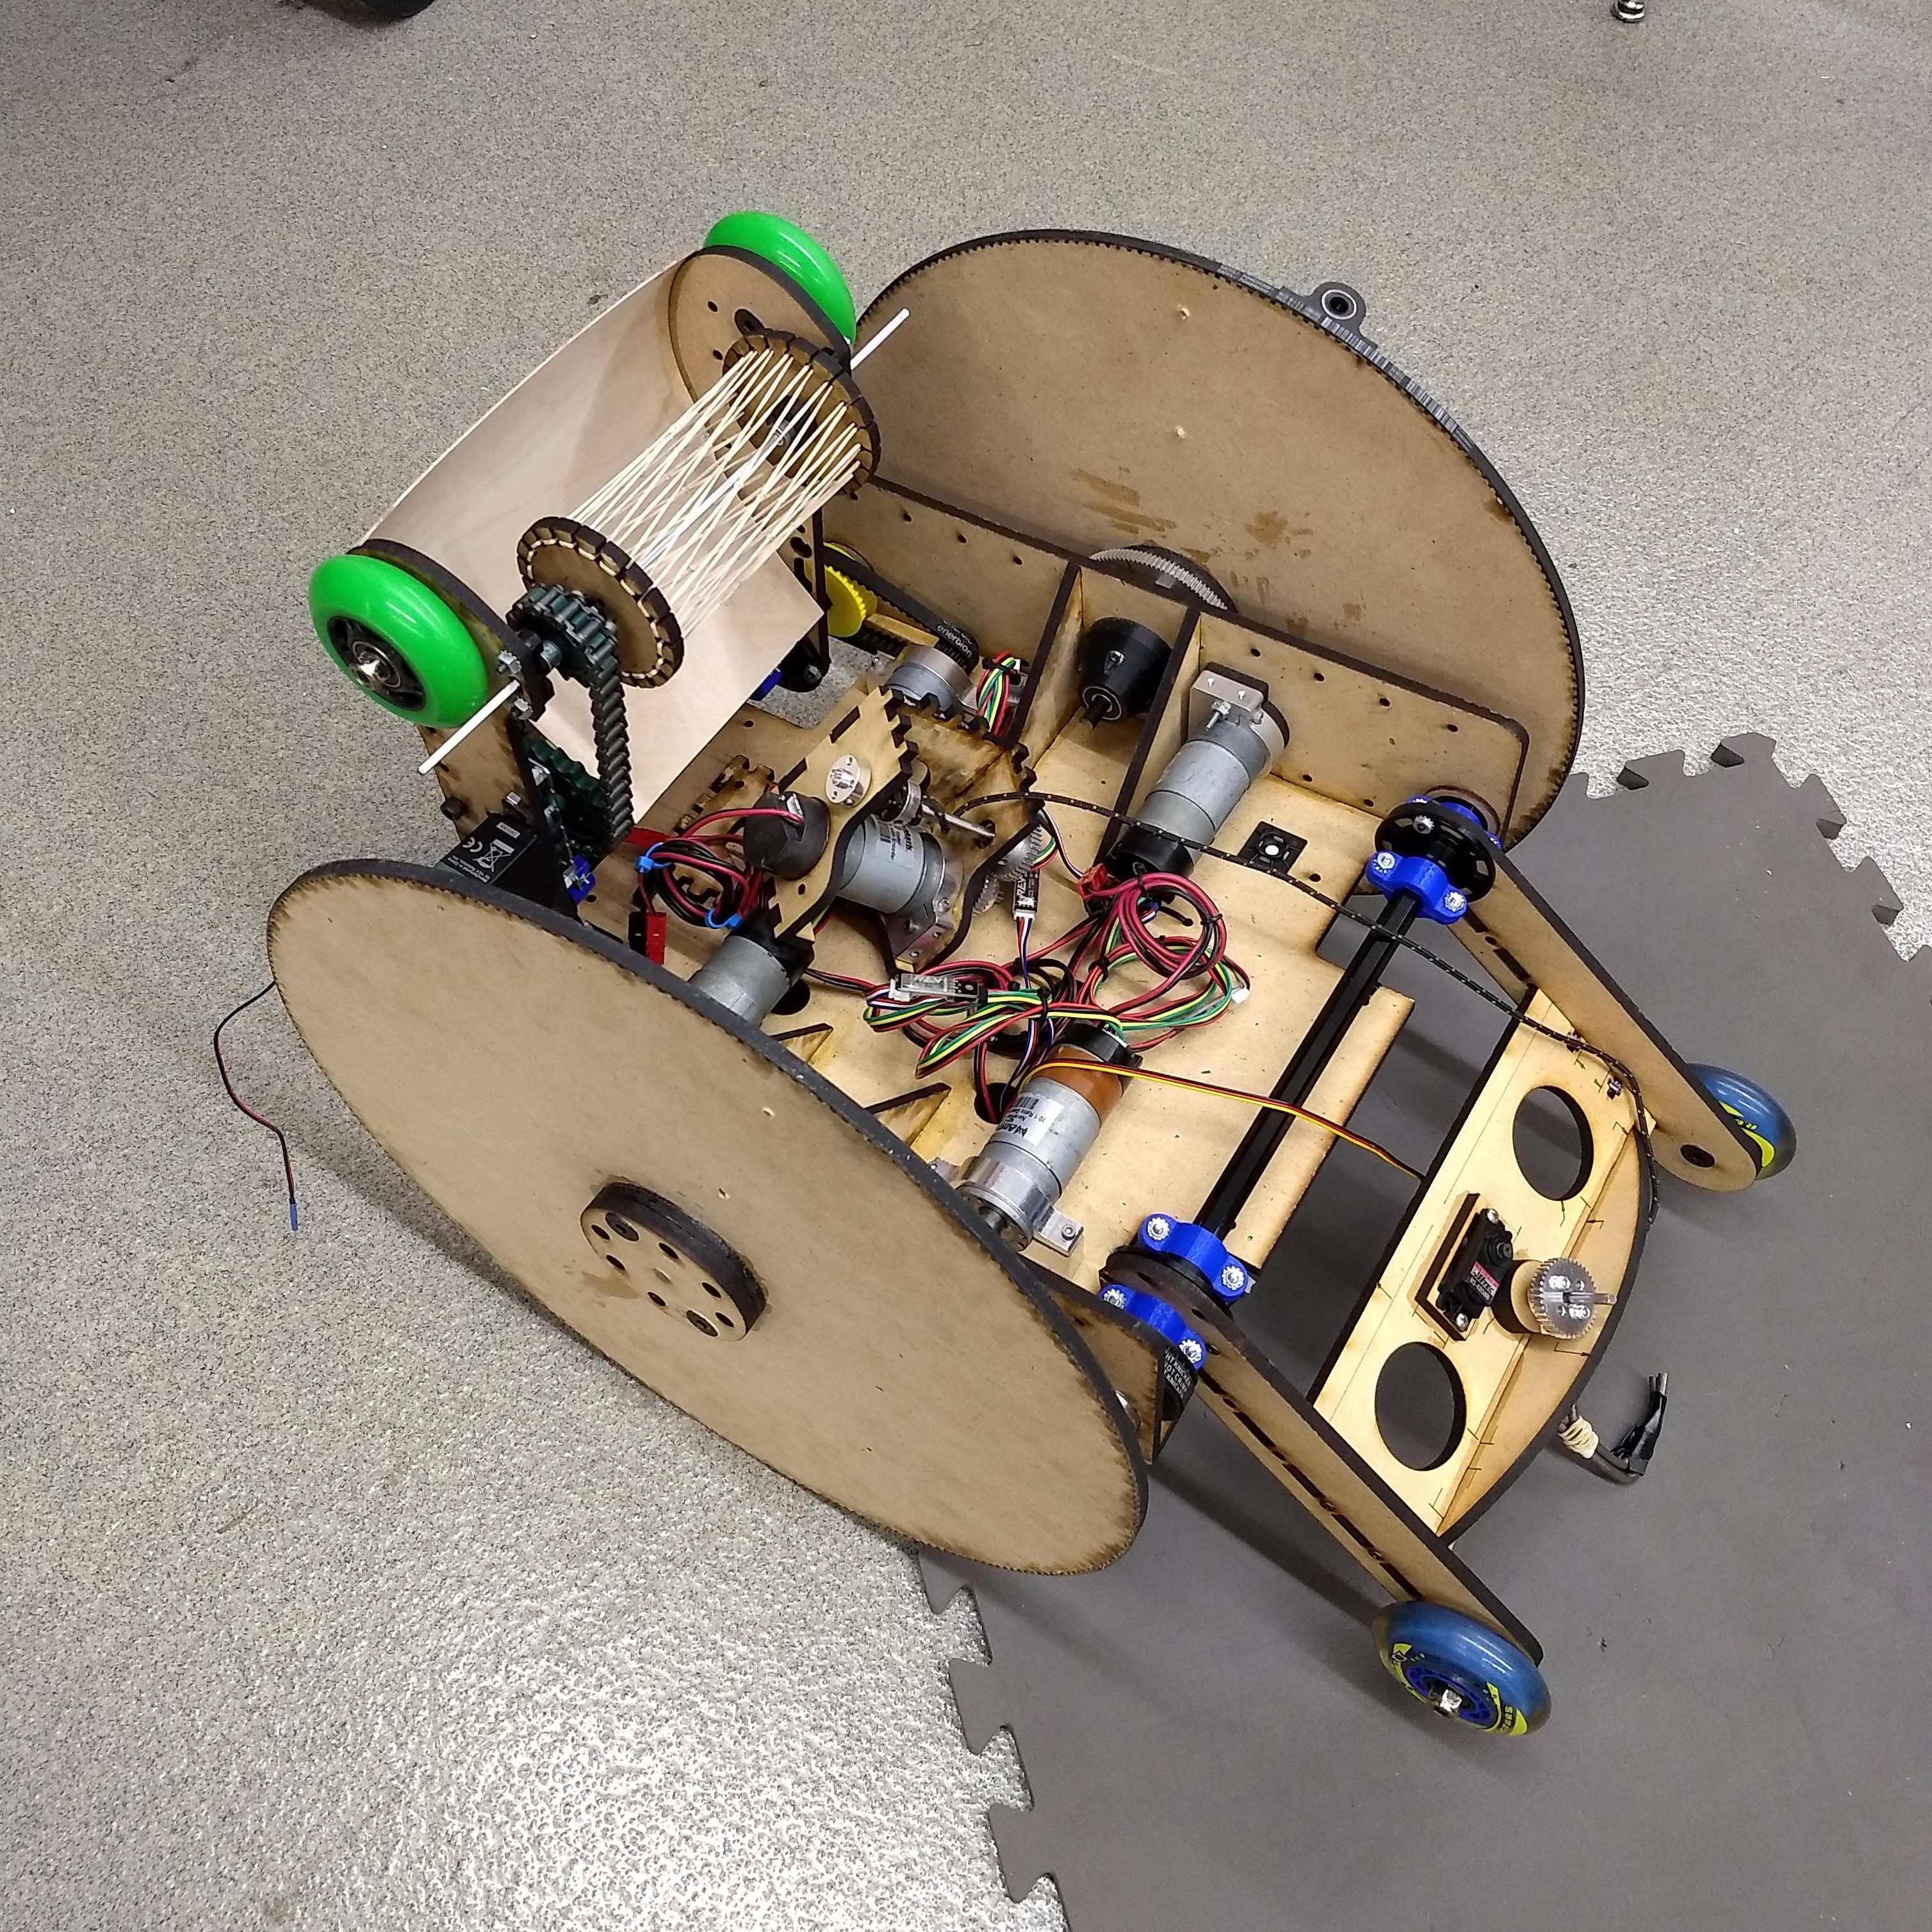
\includegraphics[width=.13\textwidth]{Design_Overview/timephoto10.jpg}
\end{center}

\end{multicols}